% lab_1.tex - Lab 1 for Cloud Computing class (Spring 2015)
% Chanmann Lim - November 2014

\documentclass[a4paper]{article}

\usepackage[margin=1 in]{geometry}
\usepackage{listings}
\usepackage{graphicx}

\begin{document}
\title{CS 7001-03: Report for Lab 1 - AWS Account Setup and Services Overview}
\author{Chanmann Lim\\ 
	\texttt{cl9p8@mail.mail.missouri.edu}}
\date{February 05, 2015}
\maketitle

\paragraph{1. } Screenshot of billing alarm setup: \\
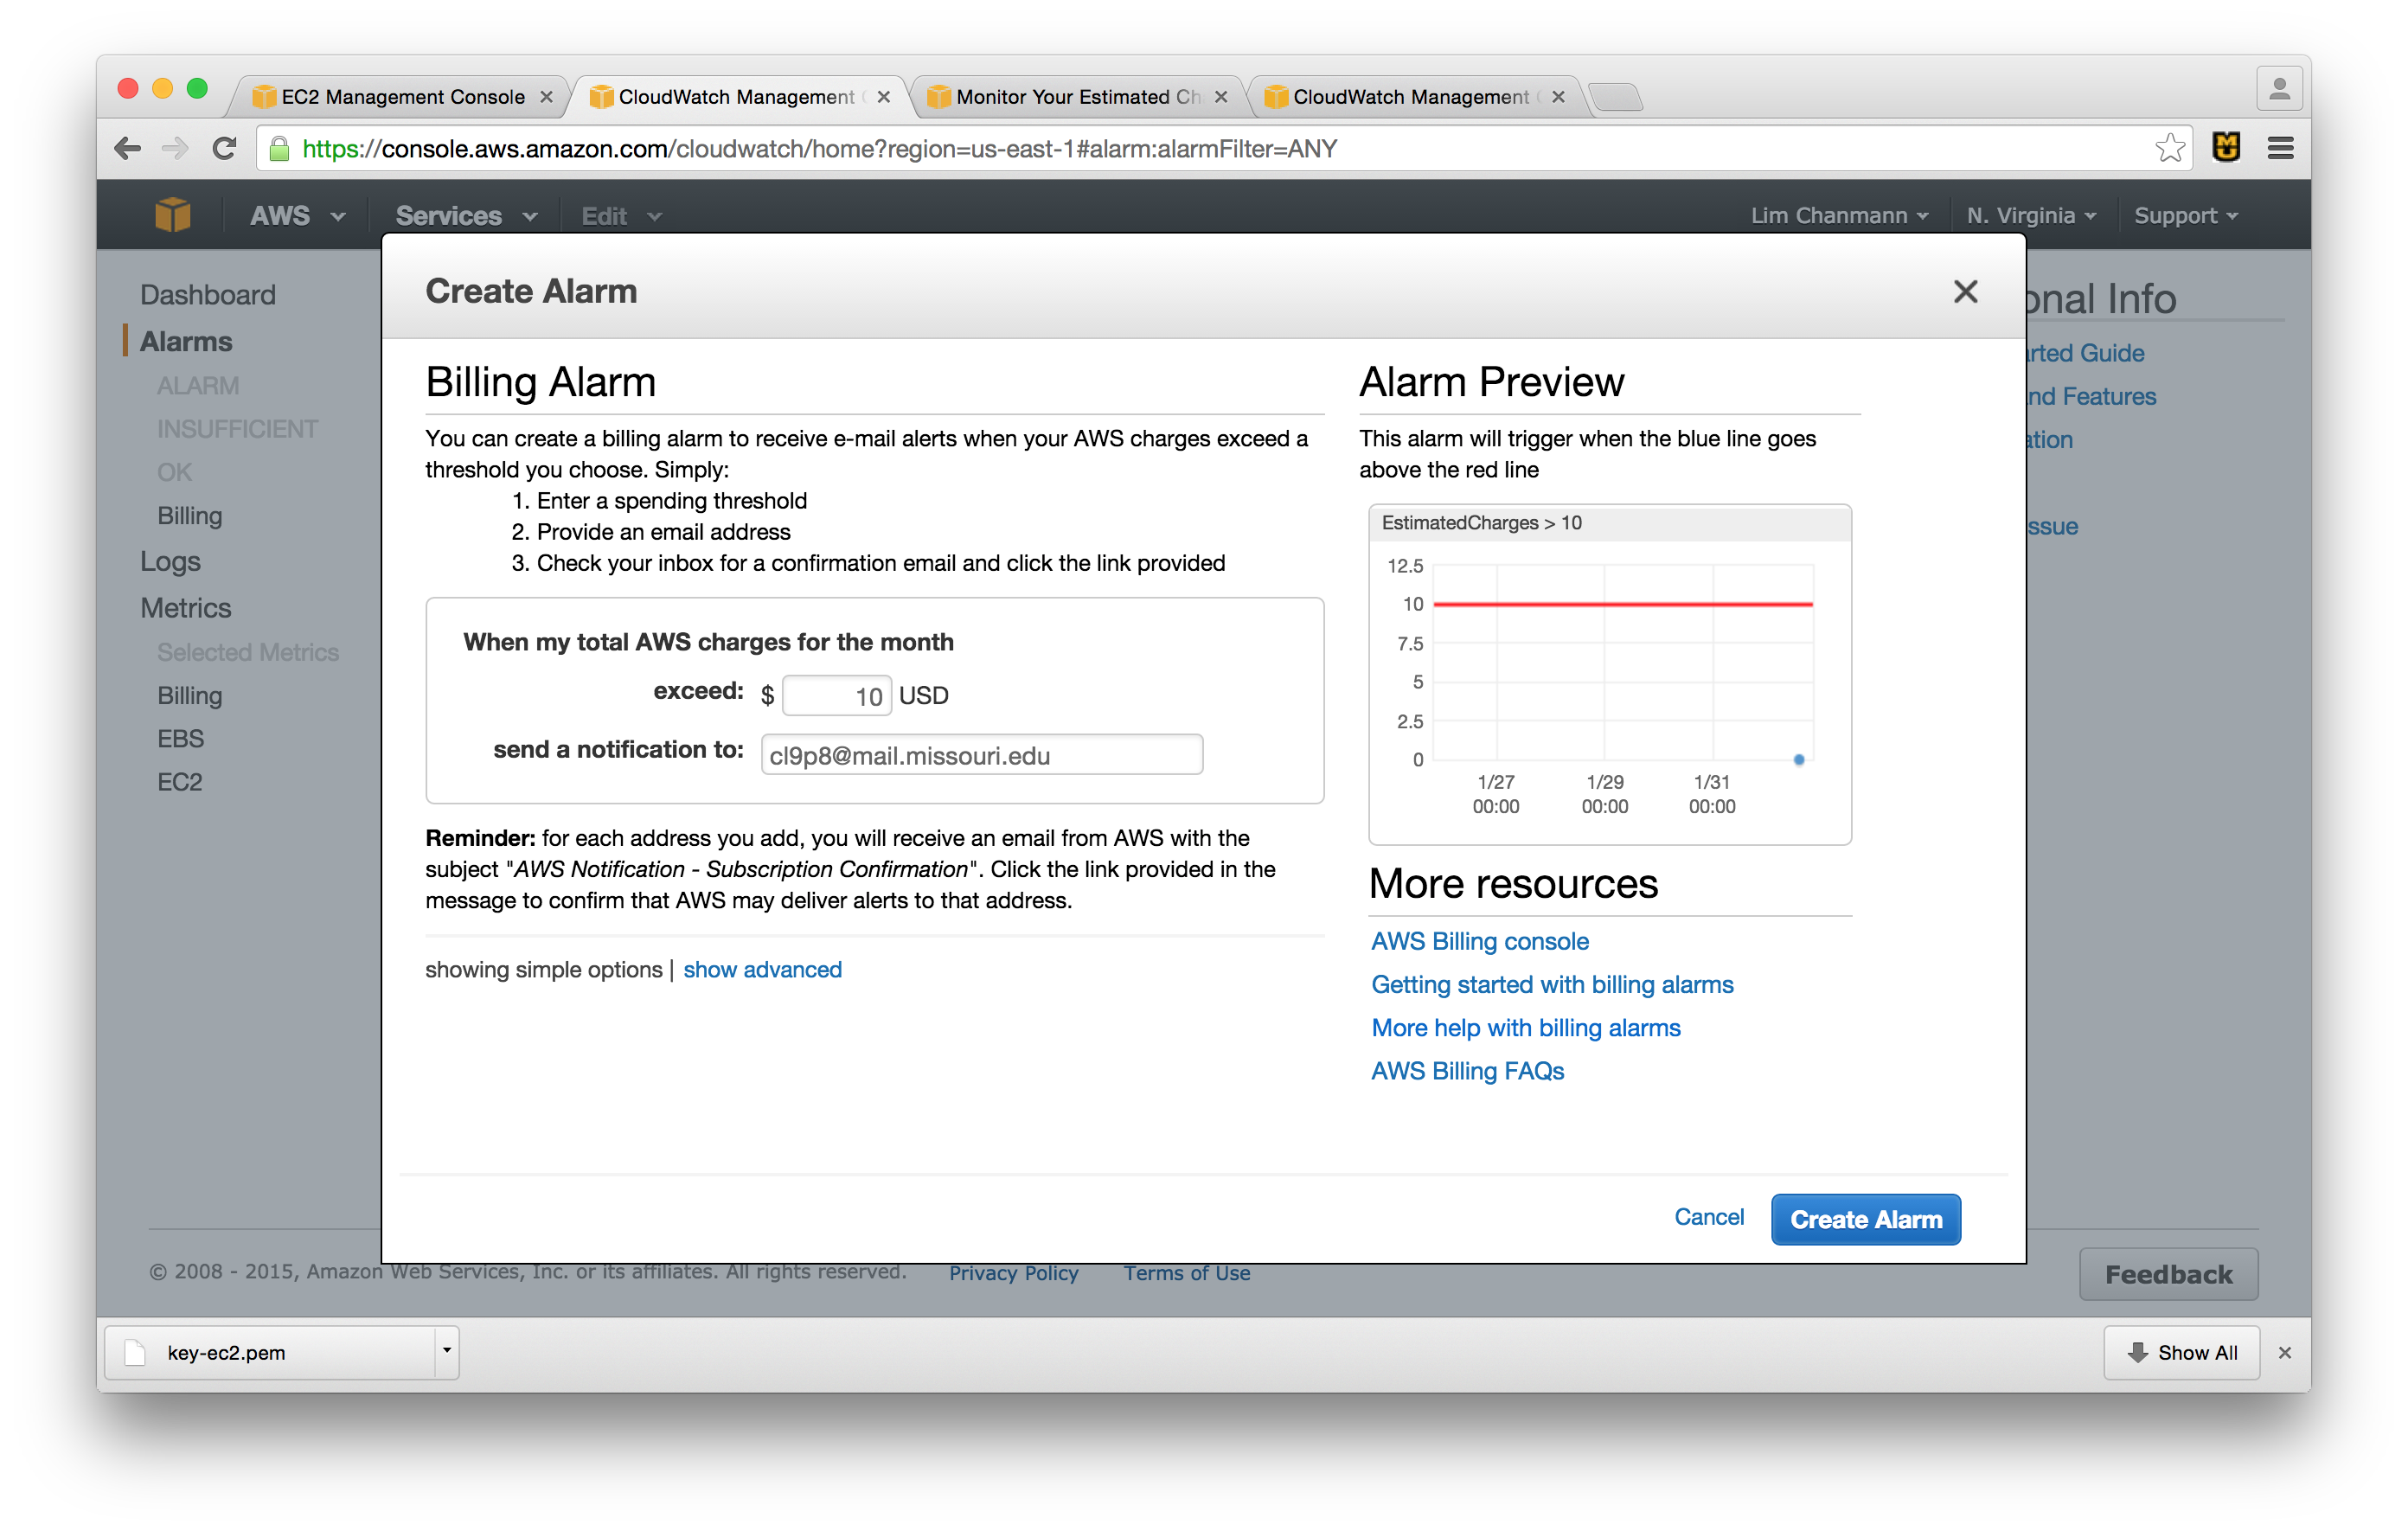
\includegraphics[scale=.32]{billing_alarm.png} \\

\paragraph{2. } List of AWS services by Categories:
\begin{description}
\leftskip 0.4in
\parindent -0.4in
	\item[Database: ] \hfill \\RDS \\DynamoDB \\ElastiCache \\RedShift
	\item[Storage \& CDN: ] \hfill \\S3 \\Storage Gateway \\Glacier \\CloudFront
	\item[Analytics: ] \hfill \\EMR \\Kinesis \\Data Pipeline
	\item[Compute \& Networking: ] \hfill \\EC2 \\VPC \\Direct Connect \\Route 53
	\item[Deployment \& Management: ] \hfill \\Elastic Beanstalk \\OpsWorks \\CloudFormation \\CodeDeploy
	\item[App Services: ] \hfill \\SQS \\AppStream \\SES \\CloudSearch
\end{description}

\paragraph{3. } Eight AWS services' objectives:
\begin{description}
\leftskip 0.4in
\parindent -0.4in
	\item[EC2 - Elastic Compute Cloud: ] \hfill \\provides scalable computing capacity (virtual servers) in Amazon Web Service cloud.
	\item[S3 - Simple Storage Service: ] \hfill \\provides files storage service.
	\item[Glacier: ] \hfill \\provides low-cost, archiving storage service.
	\item[CloudFront: ] \hfill \\provides content delivery and distribution with low latency and high data transfer speeds.
	\item[VPC - Virtual Private Could: ] \hfill \\provides networking accesses(virtual network) for user's AWS resources.
	\item[Route 53: ] \hfill \\provides Domain name system (DNS) management.
	\item[CloudWatch: ] \hfill \\provides operational and performance monitoring for AWS resources and applications.
	\item[SQS: ] \hfill \\provides message queue service for decoupling mechanism between service-to-service communication.
\end{description}

\paragraph{4. } Specification of the free instance used in the lab:
\begin{description}
\leftskip 0.4in
\parindent -0.4in
	\item[Family: ] General Purpose
	\item[Type: ] t2.micro
	\item[vCPU: ] 1 (virtual CPU 2.5 GHz Intel Xeon Family)
	\item[Memory: ] 1 (GB)
	\item[Storage: ] EBS Only (Size: 8GB, Volumn Type: Magnetic)
	\item[Network Performance: ] Low to Moderate
\end{description}

\paragraph{5. } There are other two available storage options besides "Magnetic":
\begin{description}
\leftskip 0.4in
\parindent -0.4in
	\item[General Purpose (SSD): ] provide up to 3,000 IOPS (input-output operations per second) per volume and also deliver a consistent baseline of 3 IOPS/GB.
	\item[Provisioned IOPS (SSD): ] deliver up to 4000 IOPS.
\end{description}

\paragraph{6. } According to ‘Amazon Content and Media Service Architecture’ why do IT enterprises need to use AWS to handle ‘spiky’ hour demands?

\paragraph{7. } Some AWS services have been built with fault tolerance and high availability in mind. Referring to the AWS Architecture documentation, list the services that are inherently fault tolerant and provide high availability. What other services do not inherently provide these benefits, and how does one add these capabilities within those services?

\paragraph{8. } Describe the necessity of ‘Amazon Machine Image (AMI)’ and ‘security group’ customization in ‘Web Application Hosting’ as described in the AWS Architecture documentation.























\end{document}